\section{Benchmarking framework design}
\label{des}
We discuss the design of the benchmarking framework in this section. As shown in Figure \ref{fig_design}, there are two main components of test deployment: \textit{1)} the SUT and \textit{2)} the driver. The driver has two subcomponents being \textit{i)} Data Generator and \textit{ii)} Data Queue.


\begin{figure}[h]
\centering
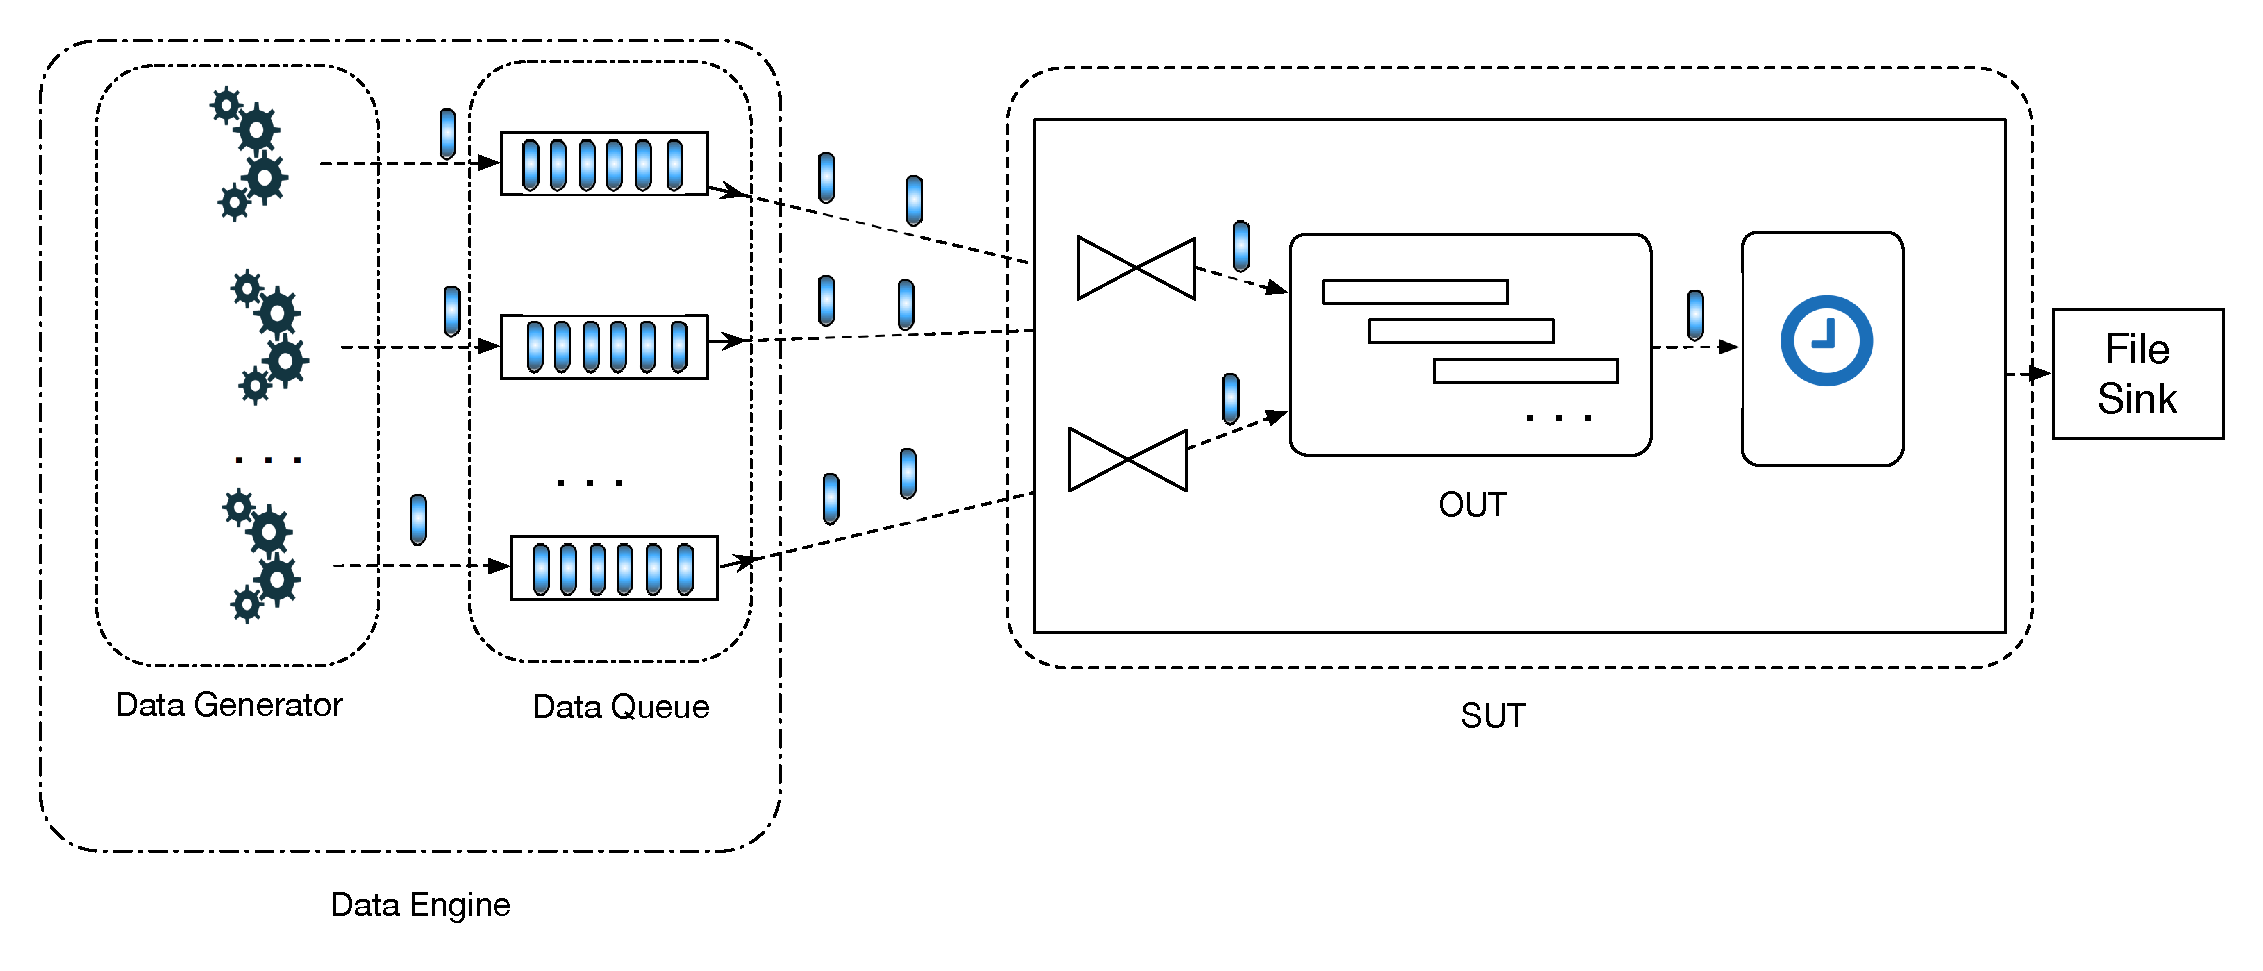
\includegraphics[width=\columnwidth]{eps/system_design}
\caption{Design of the benchmark framework.}
\label{fig_design}
\end{figure}


The Driver Instance (DI) is a combination of the Data Generator Instance (DGI) and the Data Queue Instance (DQI). %\todo[inline]{What is a slot in this setup? Please introduce the general cluster setup=>fixed} 
The driver is the combination of all DIs. Similarly, the Data Generator Subcomponent (DGS) and Data Queue Subcomponent (DQS) are the combination of all DGIs and DQIs, respectively. The driver is responsible for generating and queuing the data. It is composed of finite number of instances which are distributed evenly to the worker nodes in the cluster. The driver nodes are separate from SUT nodes in the cluster deployment. %\todo[inline]{on the same nodes as the SDPS?=>fixed}
The DGI and the DQI reside in the same machine to avoid any network overhead and to ensure data locality. The data is kept in memory to avoid disk write/read overhead. The first subcomponent, the DGS, generates data with a constant speed. Because of the bottlenecks explained in Section \ref{chal}, we avoid using mediator data queueing systems between the driver and SUT but use distributed local queues (DQS). Data is queued in first-in/first-out manner in the DQS. As explained earlier, this approach is not different from implementing centralized and distributed message queues between the SUT and the driver. The following analogy can be made: the queue topic   in a distributed message queuing system is analogous to DQS, and the queue partition is analogous to DQI. 
%\todo[inline]{A topic is not a queue, again, please be precise=>fixed}

The data generator  timestamps every event. The event's latency is calculated from this point and the longer it stays in a  queue, the higher its  latency. The number of DIs can be arbitrary and the overall throughput that can be generated is only bounded by the network bandwidth.%\todo[inline]{what is it?, the DI or the DC?=>DI is single driver instance. We dont have a bound on the number of DIs}
% \todo[inline]{How is it measured?=>explained in challenges section}

%\todo[inline]{what do you mean by outer world?=>deleted}
%\todo[inline]{Can any of the systems work with push-based sources?=>for example we could create data inside the system's source operator. This can be push based. Anyway , I deleted the  sentence.}
%. \todo[inline]{This is hard to understand, also explaining all the separation without actually explaining the measurement is confusing and from a structure point of view not good. Most of this, you already said in the challenges section. It is probably best to shorten this to the architecture part.=>deleted whole paragraph}


%Proper handling tuples' timestamp fields while joining or aggregating is crucial. In this work, \textit{merging} of tuples' timestamp fields is done by selecting \textit{maximum} over them. That is, latest arrived tuple's timestamp is transferred to the new tuple as a result of aggregation or join. Equation \ref{eq_1} defines this logic formally.
%
%
%Here $t \in T$ is a stream tuple,  $t[k]$ is  $k^{th}$ field of particular data point and $\equiv$ means equivalent in terms of type. For aggregation function $|T|$, the size of a set is not bounded, whereas for join function it is bounded by two, being $|T| = 2$.



The use-cases for this benchmark are derived from an online video game applications. Online video game companies continuously monitor the user actions in a game and ensure that the system works as expected. For example, the company tracks the number of active users and take actions on a sudden drop. Moreover, once the new feature is added to an online game or the game is updated to a new version, the company monitors the application to see  the newly added feature is working  without failures.
%\todo[inline]{Maybe change this to the use case Henri provided=>fixed}

%\textbf{Windowed Aggregation}
Windowed aggregations are an important part of the user monitoring in online video gaming. Online video game companies track the IAPs per application, per distribution channel(the application store, e.g. iTunes/appStore, Google Play), per product item (the actual IAP item like gem pack) and etc. In this benchmark, we use similar use-case monitoring the IAPs per product item. 
%\todo[inline]{Please adjust according to Henri's feedback->fixed}

%\textbf{Windowed Join}
Windowed joins are another important part of user monitoring in online video gaming.  Analysing the IAPs within a game and comparing the results based on distribution channel, user ID, and etc. is another use-case in online video game industry. In our benchmark, we get user feeds per distribution channel and compare the IAPs of the same product item between streams. That is, we divide the input streams into windows and join them per key (product item). 
%\todo[inline]{Again the same sentence as above=>fixed}
%\todo[inline]{is this relevant for us?=>fixed}


\subsection{Metrics}
The metrics for this benchmark are latency and throughput. In this section, we give the definition of each metric and explain our solution to measure it. 


%To measure the performance of a system, we connected max $16$ data generators to system under test with order of $1$,$2$,$4$,$8$ and $16$ as increasing further does not increase the overall throughput significantly. We call the tests with related workloads as $1x$, $2x$, $4x$, $8x$ and $16x$. Moreover, the configuration of each data generator must be the same. Configuration includes parameters such as overall input size, generation speed, socket port and etc. Equation \ref{eq_2} defines this formally.
%
%\begin{equation}
%  \begin{gathered}
% \textbf{Let} \ d_{i}^{c_{i}} \in  D\\
%  \textbf{then}, |D| \gets S \\
%  \textbf{and} \ c_{1} = c_{2} \ ... = c_{n}, \forall n \in S = {1,2,4,8,16}
%  \end{gathered}\label{eq_2}
%\end{equation}


\subsubsection{Throughput}

As we defined above, we use the maximum sustainable throughput to measure system's workload. Throughout the experiments, the data generation speed in all DIs are equal and constant. To examine if a system can sustain a given throughput, we divide the queue used in DQI into three parts: $q^{a}$ , $q^{b}$ and $q^{n}$. Figure \ref{fig_queue}, shows the example partitioning of the queue. If the size of the queue is less than or equal to $c^{a}$ throughout the experiment, then this is acceptable, meaning the SUT can sustain the given throughput. If the queue size is between $q^{a}$ and  $q^{b}$ on the other hand, the SUT cannot sustain the given data rate, but the driver might tolerate it for some time. A longer queue can be caused by slow system initialization, backpressure, etc. However, if the queue size is longer than $q^{b}$ then the SUT cannot sustain the given throughput and the latency is expected to continuously increase. In this case we end the experiment.

% \todo[inline]{You repeat yourself here, without explaining the sustainable throughput and the maximum throughput. Please start by explaining these before saying they are different. Probably this paragraph can be deleted completely.=>deleted all of them}

\begin{figure}[h]
\centering
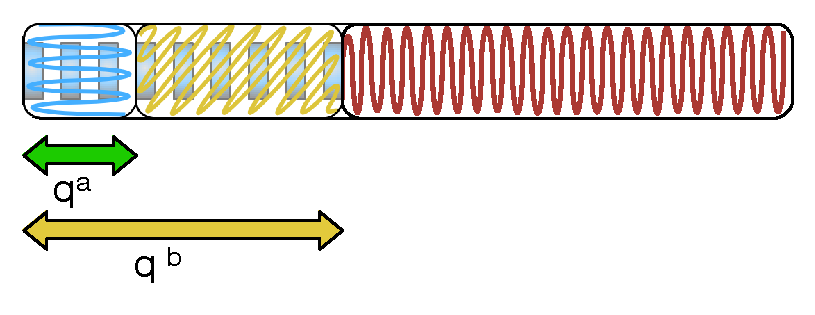
\includegraphics[width=0.5\textwidth]{eps/queue}
\caption{Basic intuition behind \textit{backpressure-compatible queue}}
\label{fig_queue}
\end{figure}
%\todo[inline]{Is this figure ever referenced in the text?=>yes}


\begin{lstlisting}[
language=SQL,
showspaces=false,
basicstyle=\ttfamily,
numbers=left,
numberstyle=\tiny,
commentstyle=\color{gray}
label={lst:label},
caption={Queries},
captionpos=b
]
S_1 = UNION  {s_1, s_2, ..., s_m}
S_2 = UNION {s_m, s_m+1, ..., s_n}
S_3 = UNION  {s_1, s_2, ..., s_n}

Query_1 = SELECT AVG(S_1.price)
FROM S_1 on window(l, s) 
GROUPBY S_1.geo

Query_2 = SELECT MAX(S_2.price, S_3.price)
FROM S_2, S_3 on window(l, s) , 
WHERE S_2.geo = S3.geo and S_2.ts = S3.ts

Query_3 = 
1.UPDATE S_1, S2: enrich with a new field = 
   cnt,  the country name of geo location
2.SELECT AVG(R.price)
  FROM  
   (SELECT MAX(S_2.price, S_3.price)
    FROM S_2, S_3 on window(l, s), 
    WHERE S_2.cnt = S3.cnt and S_2.ts = S3.ts)  
    as R on window(l, s)  
  GROUPBY R.geo
  WHERE R.price > 100




\end{lstlisting}

%The semantics behind the evaluation of a sustainable workload with a given throughput must be clear. Moreover, it should support the system specific behaviors like backpressure. 
Our system supports user-defined policies to test the sustainability. For example, one policy tolerates the $q^{b}$ part of the queue for a given time period (time based policy). Another policy tolerates   the $q^{b}$ part of the queue for a given number of pushes into the queue (count based policy).% \todo[inline]{not sure what this means=>fixed}
This policy is customizable and can be easily plugged into the driver. %\todo[inline]{DEC?=>fixed}  



We choose a policy that is a combination of time and count based policies. Once the queue size exceeds the $q^{a}$ and is less than $q^{b}$, we wait until $\frac{q^{b} - q^{a}}{2}  $ elements are pushed into the queue and check again. If the queue size is still bigger than $c^{a}$ we end the benchmark concluding the SUT cannot sustain the given throughput. %If the queue size is within $c^{a}$ and $c^{b}$, we do not tolerate it anymore. 
This process is done continuously in all DIs %\todo[inline]{DEI?=>fixed} 
and if the SUT fails to sustain one instance of the driver, then the experiments are halted meaning the SUT cannot sustain the given throughput. That is, the SUT can sustain a given workload if it can sustain the throughput of all DIs.%\todo[inline]{DEI?=>fixed}  

\textcolor{red}{ It is crucial that separation of driver and SUT and handling backpressure in the driver side does not cause side effects in metric measurements. To emplasize again, the driver does not stop the benchmark when the system exhibits backpressure. Firstly, accurate selection of $q^{a}$, $q^{b}$ and $q^{n}$ is crucial. In our experiments, first we assign 5\%, 15\% and 30\% of input size for variables $q^{a}$, $q^{b}$ and $q^{n}$ respectively. In this case, the system can "handle" the given input; however, with longer experiments it fails, as the size of the queue keeps increasing. Moreover, we get very big latencies for the given input. As a result, we keep decreasing the variables until we find the best thresholds for all systems.    Secondly, it is crucial for the driver to distinguish unsustainable throughput and backpressure. As we discussed in above paragraph, the driver can successfully handle this issue. If the queue size gets beyond $q^{a}$ and less than $q^{b}$, the driver starts to inspect the queue for the next $\frac{q^{b} - q^{a}}{2}  $ tuples. If the queue size keeps increasing, for every such tuple, then we conclude that this is not a backpressure. In fact in experiments, we show that our driver can successfully handle the backpressure.}







\subsubsection{Latency}
\label{sec_latency}
%Latency is another metric for this benchmark and  the defining of latency also needs clear semantics. There are several points that need to be clarified: \textit{i)} the aggregation or join of timestamp fields of tuples and \textit{ii)} the period  (start and end time) of latency.

%The first point is the aggregation or join of tuples with timestamp fields. 
While the use-case provides the semantics for aggregating or joining tuples, the semantics for measuring the latency of stateful operators is unclear.  We provide efficient solution for this problem in our benchmarking framework. When the tuples arrive to a stateful operator, it does the aggregation that is defined in the use-case. Besides the aggregation  defined in the use-case,  we aggregate the timestamp fields of tuples within stateful operator. That is, the timestamp of stateful operator's output tuple is the maximum timestamp of all tuples inside the operator.  The main intuition is that we exclude the tuples' waiting time in the window by taking the timestamp of the latest arrived tuple in each window. When a record is emitted from the sink operator of the SUT, we calculate the latency of a tuple by subtracting its timestamp from the current time.



\textcolor{red}{ We are aware of the fact that new definition of latency can be applied when the data is pushed to the system. }
%\todo[inline]{You define many variables here, but do not really use them. Maybe an intuitive explanation would be better.=>fixed}


%\todo[inline]{after reading this, I don't clearly understand how you measure / calculate the latency and where this is done.=>deleted}




